% To je predloga za poročila o domačih nalogah pri predmetih, katerih
% nosilec je Tomaž Curk. Avtor predloge je Blaž Zupan.
%
% Seveda lahko tudi dodaš kakšen nov, zanimiv in uporaben element,
% ki ga v tej predlogi (še) ni. Več o LaTeX-u izveš na
% spletu, na primer na http://tobi.oetiker.ch/lshort/lshort.pdf.
%
% To predlogo lahko spremeniš v PDF dokument s pomočjo programa
% pdflatex, ki je del standardne instalacije LaTeX programov.

\documentclass[a4paper,11pt]{article}
\usepackage{a4wide}
\usepackage{fullpage}
\usepackage[utf8x]{inputenc}
\usepackage[slovene]{babel}
\selectlanguage{slovene}
\usepackage[toc,page]{appendix}
\usepackage[pdftex]{graphicx} % za slike
\usepackage{setspace}
\usepackage{color}
\definecolor{light-gray}{gray}{0.95}
\usepackage{listings} % za vključevanje kode
\usepackage{hyperref}
\renewcommand{\baselinestretch}{1.2} % za boljšo berljivost večji razmak
\renewcommand{\appendixpagename}{Priloge}
\usepackage{amssymb}
\usepackage{amsmath}

\lstset{ % nastavitve za izpis kode, sem lahko tudi kaj dodaš/spremeniš
language=Python,
basicstyle=\footnotesize,
basicstyle=\ttfamily\footnotesize\setstretch{1},
backgroundcolor=\color{light-gray},
}

\title{Nenadzorovano modeliranje}
\author{Amon Stopinšek (63150273)}
\date{\today}

\begin{document}

\maketitle

\section{Uvod}
% V tem razdelku, ki naj bo kratek in naj obsega en odstavek z do 150
% besed, na kratko opišeš, kaj je bil cilj naloge.

V nalogi sem se lotil iskanja osamelcev in gruč. V prvem delu naloge sem
poiskali filme o katerih so si gledalci najmanj enotni. Problema sem se lotili
z izračunom variance za vsak film in p testa. V drugem delu naloge sem s pomočjo različnih metod poskušal poiskati filme, ki so si med seboj najbolj podobni.

\section{Podatki}

% Če je naloga zasnovana tako, da vključuje analizo izbranih podatkov, v
% tem razdelku opišeš, kakšni so ti podatki in navedeš nekaj osnovnih
% statističnih lastnosti teh podatkov. Slednje vključujejo velikost
% podatkov (na primer število primerov, število in vrsto atributov), delež
% manjkajočih podatkov, opis in porazdelitev vrednosti ciljnih
% spremenljivk, in podobno. Če si podatke pridobil sam, tu opišeš, na
% kakšen način, kje in kako.

Pri nalogi sem uporabili podatkovno zbirko
\href{https://grouplens.org/datasets/movielens/}{Movie Lens}.

\section{Metode}

% Tu opišeš, na kakšen način si rešil nalogo (tehnike in metode, ki si
% jih uporabil). Lahko vključiš tudi zanimiv del programske kode, ki
% si jo morda pri tem razvil ali pa v poročilo dodatno vključiš sliko,
% kot je na primer slika~\ref{slika1}. Vse slike in tabele, ki jih
% vključiš v poročilo, morajo biti navedene v besedilu oziroma se moraš
% na njih sklicati.
%
% \begin{figure}[htbp]
% \begin{center}
% 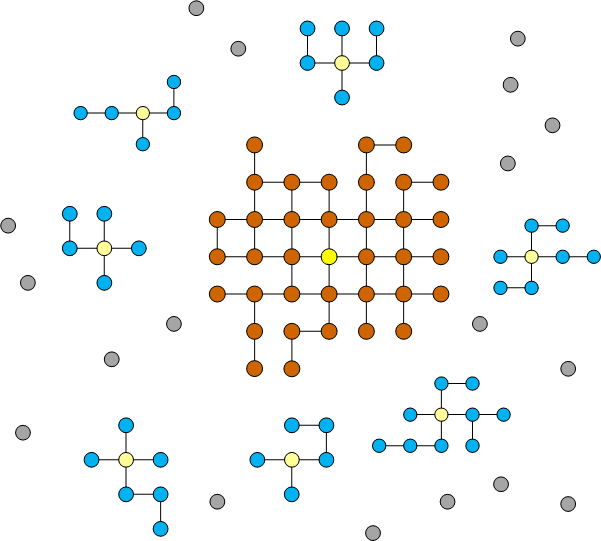
\includegraphics[scale=0.3]{slika-primer.png}
% \caption{Vsako sliko opremi s podnapisom, ki pove, kaj slika prikazuje.}
% \label{slika1}
% \end{center}
% \end{figure}
%
% V to poglavje lahko tudi vključiš kakšen metodološko zanimiv del
% kode. Primer vključitve kode oziroma implementirane funkcije v
% programskem jeziku Python je:
%
% \begin{lstlisting}
% def fib(n):
%     if n == 0:
%         return 0
%     elif n == 1:
%         return 1
%     else:
%         return fib(n-1) + fib(n-2)
% \end{lstlisting}
%
% Izris te kode je lahko sicer tudi lepši, poskušaš lahko najti še
% primernejši način vključevanja kode v Pythonu oziroma v tvojem izbranem
% programskem jeziku v okolje \LaTeX{}.

\subsection{Iskanje osamelcev}
Za iskanju osamelcev na podlagi variance ocen sem najprej preoblikoval
originalno obliko podatkov v datoteki ratings.csv v matriko\ref{tab2} kjer stolpci
predstavljajo filme, vrstice uporabnike, vrednosti pa predstavljajo oceno
filma določenega uporabnika.

\begin{lstlisting}
import pandas as pd
dfRatings = pd.read_csv('../data/ratings.csv')
df = dfRatings.pivot(index='userId', columns='movieId', values='rating')
\end{lstlisting}

\begin{table}[htbp]
\caption{Izsek iz matrike ocen}
\label{tab2}
\begin{center}
\begin{tabular}{lllllp{2cm}}
\hline
userId / movieId & 1 & 2 & 3 & 5 & 6 \\
\hline
15 & 2.0 & 2.0 & NaN & 4.5 & 4.0 \\
16 & NaN & NaN & NaN & NaN & NaN \\
17 & NaN & NaN & NaN & NaN & 4.5 \\
18 & NaN & NaN & NaN & 3.0 & 4.0 \\
19 & 3.0 & 3.0 & 3.0 & NaN & 3.0 \\
\hline
\end{tabular}
\end{center}
\end{table}

Za izračun filmov o katerih so si gledalci najmanj enotni sem uporabil varianco. Izračun variance ocen vsakega filma je bil zaradi oblike podatkov in uporabe knjižice \href{http://pandas.pydata.org/index.html}{pandas} precej preprost.

\begin{lstlisting}
df.var()
\end{lstlisting}

Pri prikazu porazdelitve izračunanih varianc so lepo porazdelitev "pokvarili"\ref{slika1}\hspace{0cm} filmi z malo ocenami. Problem sem rešil tako, da sem izločili filme z manj kot 10 ocenami. Za iskanje osamelcev je s tem ostalo 2245 filmov.

\begin{lstlisting}
df = df.dropna(axis=1, how='any', thresh=10, subset=None, inplace=False)
\end{lstlisting}

\begin{figure}[htbp]
\begin{center}
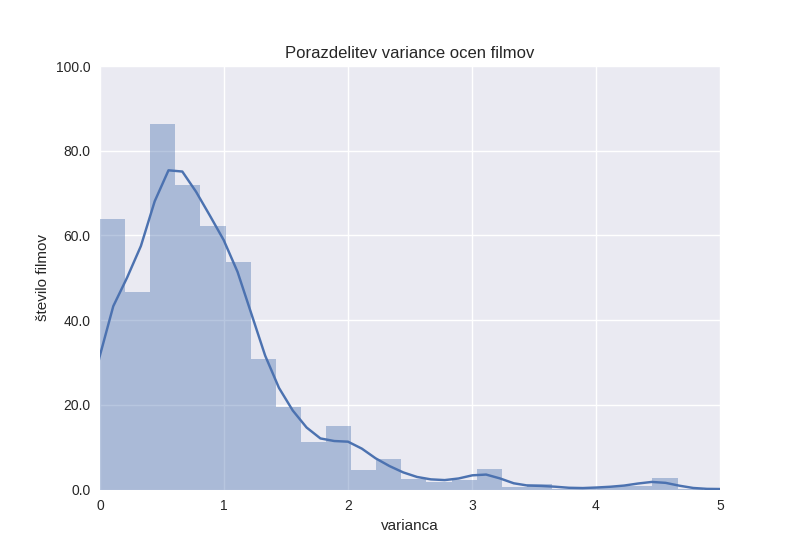
\includegraphics[scale=0.7]{porazdelitevPrva.png}
\caption{Porazdelitev variance filmov brez izločanja filmov z malo ocenami}
\label{slika1}
\end{center}
\end{figure}

\subsection{Gručenje filmov}
Iskanja skupin med filmi sem se lotil na podoben način kot iskanja osamelcev. Iz podatkov sem najprej sestavil matriko
film / uporabnik.

Gručenja sem se najprej lotil z metodo k-Means. Preizkusil sem različne možnosti za izračun razdalje (evklidska, manhatenska, razdalja je 1 - presek uporabnikov, ki so ocenili oba filma deljeno z unijo uporabnikov, ki so ocenili vsaj enega izmed filmov, ...). Najbolje se je izkazala evklidska razdalja, tudi z uporabo le te pa so bili rezultati gručenja še vedno neuporabni.

Zaradi slabih rezultatov z metodo k-means sem za gručenje preizkusil še metodo DBSCAN. Tudi uporaba te metode se ni izkazala za uspešno, vse filme je označila kot šum, ali pa vsak film razvrstila v svojo skupino.

Preizkusil sem še hirearhično gručenje z wardovo metodo. Slika \ref{slika7} prikazuje dobljeni dendogram. Tudi ta metoda se ni izkazala z uporabnimi rezultati.

Podatke sem izvozil še v format .xslx in jih uporabil v programu Orange. Tudi tam mi ni uspelo iz danih podatkov poiskati dobrih skupin z uporabo metod k-means in hirearhičnega razvrščanja.

\section{Rezultati}

% V tem poglavju podaš rezultate s kratkim (enoodstavčnim)
% komentarjem. Rezultate lahko prikažeš tudi v tabeli (primer je
% tabela~\ref{tab1}).

% Odstavke pri pisanju poročila v LaTeX-u ločiš tako, da pred novim
% odstavkom pustiš prazno vrstico. Tudi, če pišeš poročilo v kakšnem
% drugem urejevalniku, morajo odstavki biti vidno ločeni. To narediš z
% zamikanjem ali pa z dodatnim presledkom.

% \begin{table}[htbp]
% \caption{Atributi in njihove zaloge vrednosti.}
% \label{tab1}
% \begin{center}
% \begin{tabular}{llp{3cm}}
% \hline
% ime spremenljivke & definicijsko območje & opis \\
% \hline
% cena & [0, 500] & cena izdelka v EUR\\
% teža & [1, 1000] & teža izdelka v dag \\
% kakovost & [slaba|srednja|dobra] & kakovost izdelka \\
% \hline
% \end{tabular}
% \end{center}
% \end{table}

% Podajanje rezultati naj bo primerno strukturirano. Če ima naloga več
% podnalog, uporabi podpoglavja. Če bi želel poročati o rezultatih
% izčrpno in pri tem uporabiti vrsto tabel ali grafov, razmisli o
% varianti, kjer v tem poglavju prikažeš in komentiraš samo glavne
% rezultate, kakšne manj zanimive detajle pa vključite v prilogo (glej
% prilogi~\ref{app-res} in~\ref{app-code}).
\subsection{Iskanje osamelcev}
Na vprašanje kateri filmi imajo najbolj razpršene ocene odgovori varianca ocen posameznega filma. 

Graf\ref{slika2} prikazuje kako so porazdeljene variance ocen vseh filmov z več kot 10 ocenami.

\begin{figure}[htbp]
\begin{center}
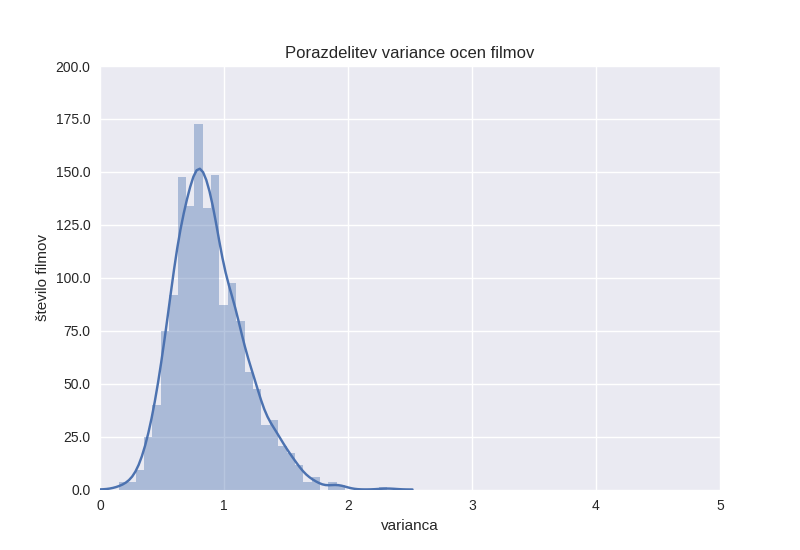
\includegraphics[scale=0.7]{porazdelitev.png}
\caption{Porazdelitev varianc ocen filmov}
\label{slika2}
\end{center}
\end{figure}

Dobljena porazdelitev precej odstopa od normalne\ref{slika2}. Od porazdelitev, ki smo jih spoznali porazdelitvi še najbolje ustreza porazdelitev beta. Izračunani oceni parametrov za beta porazdelitev so:
\begin{lstlisting}
params = stats.beta.fit(x)
print(params)
> (6.90759787872952, 27.9450733031308, -0.11751603359648, 5.1490259125502)
\end{lstlisting}


Na grafu\ref{slika5}, ki ima dorisano še krivuljo beta porazdelitve lahko primerjamo ujemanje beta porazdelitve z dejansko.

Preizkusil sem še nekaj ostalih porazdelitev. Za najboljšo se je izkazala \href{https://en.wikipedia.org/wiki/Noncentral_t-distribution}{Noncentral t-distribution}\ref{slika4}. 


\begin{figure}[htbp]
\begin{center}
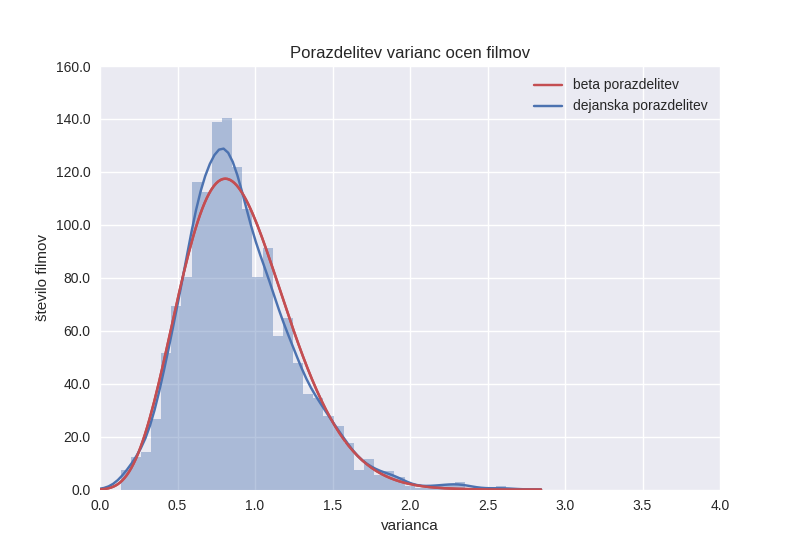
\includegraphics[scale=0.7]{porazdelitevBeta.png}
\caption{Primerjava krivulje porazdelitve z Beta}
\label{slika5}
\end{center}
\end{figure}


V zgornjih 5\% statistično najbolj značilnih filmov spada 133 filmov od 2245. Tabela\ref{tab3} prikazuje 10 filmov, ki so med vsemi najbolj izstopali.


\begin{table}[htbp]
\caption{10 najbolj statistično značilnih filmov}
\label{tab3}
\begin{center}
\begin{tabular}{lp{2cm}}
\hline
naslov filma & varianca \\
\hline
Killing Zoe (1994) & 2.620\\
Dead Man (1995) & 2.558 \\
Christmas Carol, A (1938) & 2.428\\
Cook the Thief His Wife \& Her Lover, The (1989) & 2.372 \\
Stalker (1979) & 2.323\\
Event Horizon (1997) & 2.322 \\
Great Expectations (1998) & 2.317 \\
Dungeons \& Dragons (2000) & 2.316 \\
The Hunger Games: Mockingjay - Part 1 (2014) & 2.281 \\
Deadpool (2016) & 2.273 \\
\hline
\end{tabular}
\end{center}
\end{table}

\subsection{Gručenje filmov}
Za gručenje filmov sem izbral metode k-means, dbscan in hirearhično razvrščanje. Za mero podobnosti sem uporabil evklidsko in manhatensko razdaljo ter wardovo metodo. Poleg naštetih sem podobnost meril tudi z razmerjem med številom uporabnikov ki so ocenili oba filma in unijo uporabnikov, ki so ocenili vsaj enega izmed filmov.

Izbran nabor algoritmov za gručenje in mer podobnosti težko utemeljim, saj so se vsi izkazali za neuporabne za dani problem.

Med izbranimi filmi je 53 skupin, če privzamemo, da je vsaka kombinacija žanrov svoja skupina. Če upoštevamo samo prvo napisano kategorijo, pa izbrani filmi spadajo v 11 različnih skupin\ref{tab4}. Štirje filmi izmed izbranih filmov nimajo določenega žanra.

Obstaja veliko metod in ocen za ocenitev kvalitete razvrščanja v gruče kot so naprimer silhouette, dunn's index, Krzanowski-Lai index, R-square,..

Za validacijo gručenja sem uporabil silhouette score, ki omogoča še vizualizacijo ocene. Ocenil sem dobljene gruče, ki sem jih dobil po uporabi metode k-means\ref{slika5} in hirearhičnega razvrščanja\ref{slika6}.



\begin{figure}[htbp]
\begin{center}
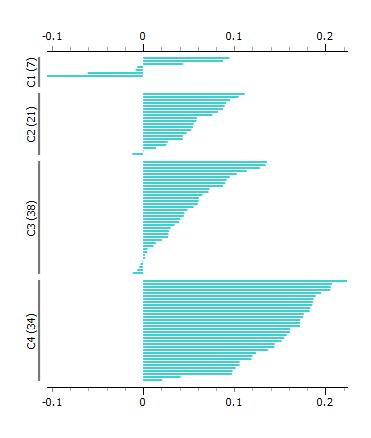
\includegraphics[scale=0.7]{k-means-silhuette.png}
\caption{K-means silhuette}
\label{slika5}
\end{center}
\end{figure}

\begin{figure}[htbp]
\begin{center}
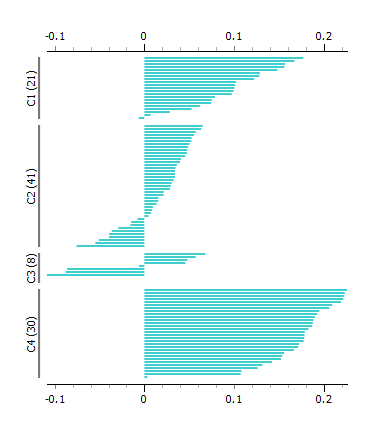
\includegraphics[scale=0.7]{hirearhicno-silhuette.png}
\caption{silhuette score za hirearhično razvrščanje}
\label{slika6}
\end{center}
\end{figure}


Dobljeni rezultati so zelo slabi. Gruče delujejo zelo naključno v primerjavi s pravimi žanri. Tudi dobljena ocena silhouette je bila v obeh primerih zelo nizka, pri hirearhičnem razvrščanju ima veliko filmov tudi negativno silhuette oceno, kar pomeni, da niso podobni ostalim filmom v svojem razredu.

\section{Izjava o izdelavi domače naloge}
Domačo nalogo in pripadajoče programe sem izdelal sam.

\appendix
\appendixpage
\section{\label{app-res}Podrobni rezultati poskusov}

% Če je rezultatov v smislu tabel ali pa grafov v nalogi mnogo,
% predstavi v osnovnem besedilu samo glavne, podroben prikaz
% rezultatov pa lahko predstaviš v prilogi. V glavnem besedilu ne
% pozabi navesti, da so podrobni rezultati podani v prilogi.

\begin{figure}[htbp]
\begin{center}
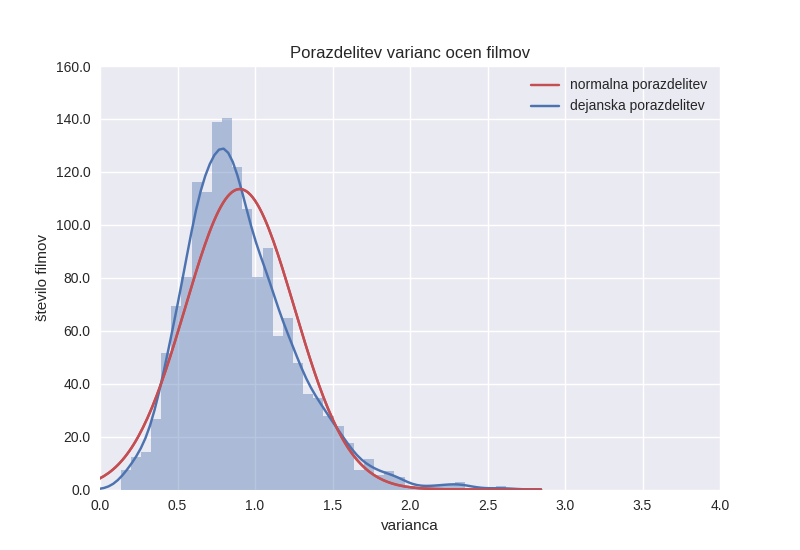
\includegraphics[scale=0.7]{porazdelitevNormalna.png}
\caption{Primerjava dejanske krivulje porazdelitve in krivulje normalne porazdelitve}
\label{slika3}
\end{center}
\end{figure}


\begin{figure}[htbp]
\begin{center}
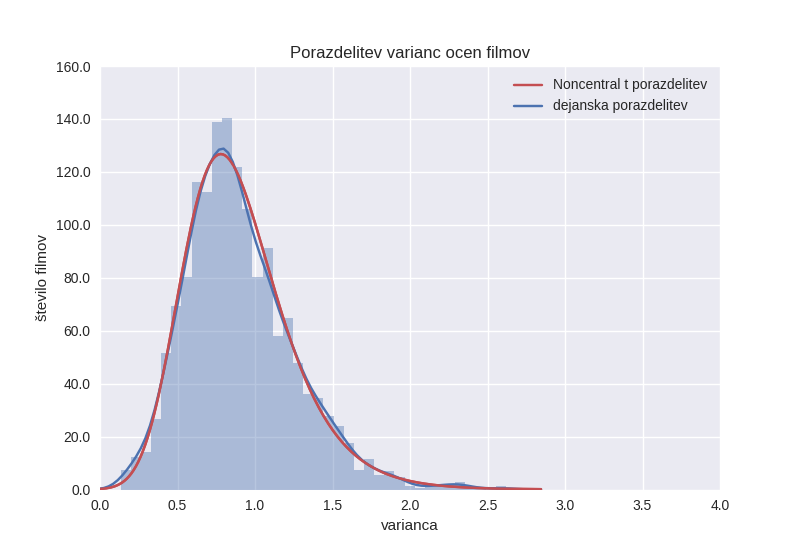
\includegraphics[scale=0.7]{porazdelitevStudent.png}
\caption{Primerjava krivulje porazdelitve z Noncentral t-distribution}
\label{slika4}
\end{center}
\end{figure}

\begin{figure}[htbp]
\begin{center}
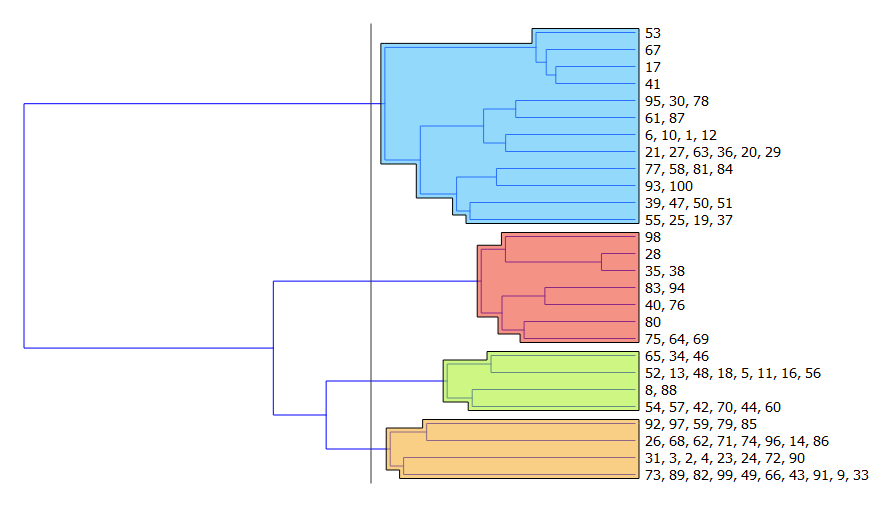
\includegraphics[scale=0.7]{hirearhicno.png}
\caption{hirearhično razvrščanje}
\label{slika7}
\end{center}
\end{figure}

\begin{table}[htbp]
\caption{Število filmov v posamezni kategoriji}
\label{tab4}
\begin{center}
\begin{tabular}{lp{2cm}}
\hline
žanr & število filmov \\
\hline

Comedy      & 28 \\  
Drama       & 22 \\  
Action      & 18 \\  
Crime       & 12 \\  
Horror      &  6 \\  
Adventure   &  5 \\  
Animation   &  1 \\  
Documentary &  1 \\  
Mystery     &  1 \\  
Romance     &  1 \\  
Thriller    &  1 \\ 
\hline
\end{tabular}
\end{center}
\end{table}

\section{\label{app-code}Programska koda}

% Za domače naloge bo tipično potrebno kaj sprogramirati. Celotno kodo oddaj
% zapakirano skupaj s poročilom v datoteki zip. V kolikor je določen izsek kode
% nujen za boljše razumevanje poročila, ga vključi v prilogo poročila.

% Čisto
% za okus sem tu postavil nekaj kode, ki uporablja Orange
% (\url{http://www.biolab.si/orange}) in razvrščanje v skupine.


% \begin{lstlisting}
% import random
% import Orange

% data_names = ["iris", "housing", "vehicle"]
% data_sets = [Orange.data.Table(name) for name in data_names]

% print "%10s %3s %3s %3s" % ("", "Rnd", "Div", "HC")
% for data, name in zip(data_sets, data_names):
%     random.seed(42)
%     km_random = Orange.clustering.kmeans.Clustering(data, centroids = 3)
%     km_diversity = Orange.clustering.kmeans.Clustering(data, centroids = 3,
%         initialization=Orange.clustering.kmeans.init_diversity)
%     km_hc = Orange.clustering.kmeans.Clustering(data, centroids = 3,
%         initialization=Orange.clustering.kmeans.init_hclustering(n=100))
%     print "%10s %3d %3d %3d" % (name, km_random.iteration, \
%     km_diversity.iteration, km_hc.iteration)
% \end{lstlisting}

\end{document}
